

\tikzset{every picture/.style={line width=0.75pt}} %set default line width to 0.75pt        

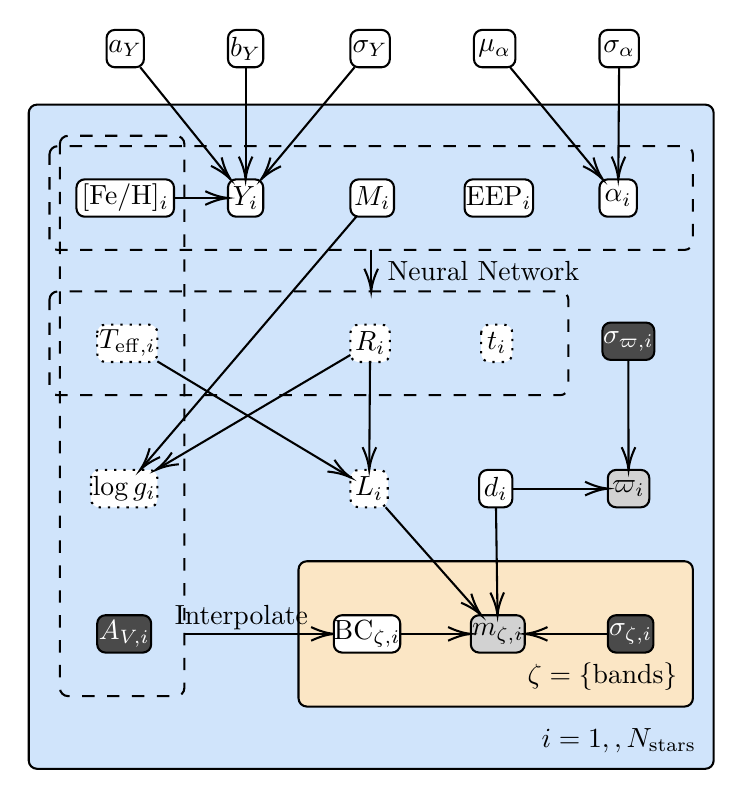
\begin{tikzpicture}[x=0.75pt,y=0.75pt,yscale=-1,xscale=1]
%uncomment if require: \path (0,444); %set diagram left start at 0, and has height of 444

%Shape: Rectangle [id:dp8264155433429197] 
\draw  [fill={rgb, 255:red, 208; green, 228; blue, 251 }  ,fill opacity=1 ] (80,84) .. controls (80,81.79) and (81.79,80) .. (84,80) -- (406,80) .. controls (408.21,80) and (410,81.79) .. (410,84) -- (410,396) .. controls (410,398.21) and (408.21,400) .. (406,400) -- (84,400) .. controls (81.79,400) and (80,398.21) .. (80,396) -- cycle ;
%Shape: Rectangle [id:dp5062275165485008] 
\draw  [dash pattern={on 4.5pt off 4.5pt}] (90,104) .. controls (90,101.79) and (91.79,100) .. (94,100) -- (396,100) .. controls (398.21,100) and (400,101.79) .. (400,104) -- (400,146) .. controls (400,148.21) and (398.21,150) .. (396,150) -- (94,150) .. controls (91.79,150) and (90,148.21) .. (90,146) -- cycle ;
%Shape: Rectangle [id:dp9697742104394034] 
\draw  [dash pattern={on 4.5pt off 4.5pt}] (90,174) .. controls (90,171.79) and (91.79,170) .. (94,170) -- (336,170) .. controls (338.21,170) and (340,171.79) .. (340,174) -- (340,216) .. controls (340,218.21) and (338.21,220) .. (336,220) -- (94,220) .. controls (91.79,220) and (90,218.21) .. (90,216) -- cycle ;
%Shape: Rectangle [id:dp8454671375857623] 
\draw  [dash pattern={on 4.5pt off 4.5pt}] (95,99) .. controls (95,96.79) and (96.79,95) .. (99,95) -- (151,95) .. controls (153.21,95) and (155,96.79) .. (155,99) -- (155,361) .. controls (155,363.21) and (153.21,365) .. (151,365) -- (99,365) .. controls (96.79,365) and (95,363.21) .. (95,361) -- cycle ;
%Shape: Rectangle [id:dp6418896844809463] 
\draw  [fill={rgb, 255:red, 251; green, 230; blue, 197 }  ,fill opacity=1 ] (210,304) .. controls (210,301.79) and (211.79,300) .. (214,300) -- (396,300) .. controls (398.21,300) and (400,301.79) .. (400,304) -- (400,366) .. controls (400,368.21) and (398.21,370) .. (396,370) -- (214,370) .. controls (211.79,370) and (210,368.21) .. (210,366) -- cycle ;
%Straight Lines [id:da13559191728628717] 
\draw    (245,150) -- (245,168) ;
\draw [shift={(245,170)}, rotate = 270] [color={rgb, 255:red, 0; green, 0; blue, 0 }  ][line width=0.75]    (10.93,-3.29) .. controls (6.95,-1.4) and (3.31,-0.3) .. (0,0) .. controls (3.31,0.3) and (6.95,1.4) .. (10.93,3.29)   ;
%Straight Lines [id:da92160867280711] 
\draw    (155,335) -- (225,335) ;
\draw [shift={(227,335)}, rotate = 180] [color={rgb, 255:red, 0; green, 0; blue, 0 }  ][line width=0.75]    (10.93,-3.29) .. controls (6.95,-1.4) and (3.31,-0.3) .. (0,0) .. controls (3.31,0.3) and (6.95,1.4) .. (10.93,3.29)   ;

% Text Node
\draw  [fill={rgb, 255:red, 255; green, 255; blue, 255 }  ,fill opacity=1 ]  (176,120) .. controls (176,117.79) and (177.79,116) .. (180,116) -- (189,116) .. controls (191.21,116) and (193,117.79) .. (193,120) -- (193,130) .. controls (193,132.21) and (191.21,134) .. (189,134) -- (180,134) .. controls (177.79,134) and (176,132.21) .. (176,130) -- cycle  ;
\draw (184.5,125) node   [align=left] {$\displaystyle Y_{i}$};
% Text Node
\draw  [fill={rgb, 255:red, 255; green, 255; blue, 255 }  ,fill opacity=1 ]  (103,120) .. controls (103,117.79) and (104.79,116) .. (107,116) -- (146,116) .. controls (148.21,116) and (150,117.79) .. (150,120) -- (150,130) .. controls (150,132.21) and (148.21,134) .. (146,134) -- (107,134) .. controls (104.79,134) and (103,132.21) .. (103,130) -- cycle  ;
\draw (126.5,125) node   [align=left] {$\displaystyle [\mathrm{Fe/H}]_{i}$};
% Text Node
\draw  [fill={rgb, 255:red, 255; green, 255; blue, 255 }  ,fill opacity=1 ]  (235,120) .. controls (235,117.79) and (236.79,116) .. (239,116) -- (252,116) .. controls (254.21,116) and (256,117.79) .. (256,120) -- (256,130) .. controls (256,132.21) and (254.21,134) .. (252,134) -- (239,134) .. controls (236.79,134) and (235,132.21) .. (235,130) -- cycle  ;
\draw (245.5,125) node   [align=left] {$\displaystyle M_{i}$};
% Text Node
\draw  [fill={rgb, 255:red, 255; green, 255; blue, 255 }  ,fill opacity=1 ]  (290,120) .. controls (290,117.79) and (291.79,116) .. (294,116) -- (319,116) .. controls (321.21,116) and (323,117.79) .. (323,120) -- (323,130) .. controls (323,132.21) and (321.21,134) .. (319,134) -- (294,134) .. controls (291.79,134) and (290,132.21) .. (290,130) -- cycle  ;
\draw (306.5,125) node   [align=left] {$\displaystyle \mathrm{EEP}_{i}$};
% Text Node
\draw  [fill={rgb, 255:red, 255; green, 255; blue, 255 }  ,fill opacity=1 ]  (355,120) .. controls (355,117.79) and (356.79,116) .. (359,116) -- (369,116) .. controls (371.21,116) and (373,117.79) .. (373,120) -- (373,130) .. controls (373,132.21) and (371.21,134) .. (369,134) -- (359,134) .. controls (356.79,134) and (355,132.21) .. (355,130) -- cycle  ;
\draw (364,125) node   [align=left] {$\displaystyle \alpha _{i}$};
% Text Node
\draw  [fill={rgb, 255:red, 255; green, 255; blue, 255 }  ,fill opacity=1 ][dash pattern={on 0.84pt off 2.51pt}]  (110,260) .. controls (110,257.79) and (111.79,256) .. (114,256) -- (138,256) .. controls (140.21,256) and (142,257.79) .. (142,260) -- (142,270) .. controls (142,272.21) and (140.21,274) .. (138,274) -- (114,274) .. controls (111.79,274) and (110,272.21) .. (110,270) -- cycle  ;
\draw (126,265) node   [align=left] {$\displaystyle \log g_{i}$};
% Text Node
\draw  [fill={rgb, 255:red, 255; green, 255; blue, 255 }  ,fill opacity=1 ][dash pattern={on 0.84pt off 2.51pt}]  (113,190) .. controls (113,187.79) and (114.79,186) .. (117,186) -- (138,186) .. controls (140.21,186) and (142,187.79) .. (142,190) -- (142,200) .. controls (142,202.21) and (140.21,204) .. (138,204) -- (117,204) .. controls (114.79,204) and (113,202.21) .. (113,200) -- cycle  ;
\draw (127.5,195) node   [align=left] {$\displaystyle T_{\mathrm{eff} ,i}$};
% Text Node
\draw  [fill={rgb, 255:red, 255; green, 255; blue, 255 }  ,fill opacity=1 ][dash pattern={on 0.84pt off 2.51pt}]  (235,190) .. controls (235,187.79) and (236.79,186) .. (239,186) -- (250,186) .. controls (252.21,186) and (254,187.79) .. (254,190) -- (254,200) .. controls (254,202.21) and (252.21,204) .. (250,204) -- (239,204) .. controls (236.79,204) and (235,202.21) .. (235,200) -- cycle  ;
\draw (244.5,195) node   [align=left] {$\displaystyle R_{i}$};
% Text Node
\draw  [fill={rgb, 255:red, 255; green, 255; blue, 255 }  ,fill opacity=1 ][dash pattern={on 0.84pt off 2.51pt}]  (298,190) .. controls (298,187.79) and (299.79,186) .. (302,186) -- (309,186) .. controls (311.21,186) and (313,187.79) .. (313,190) -- (313,200) .. controls (313,202.21) and (311.21,204) .. (309,204) -- (302,204) .. controls (299.79,204) and (298,202.21) .. (298,200) -- cycle  ;
\draw (305.5,195) node   [align=left] {$\displaystyle t_{i}$};
% Text Node
\draw  [fill={rgb, 255:red, 74; green, 74; blue, 74 }  ,fill opacity=1 ]  (113,330) .. controls (113,327.79) and (114.79,326) .. (117,326) -- (135,326) .. controls (137.21,326) and (139,327.79) .. (139,330) -- (139,340) .. controls (139,342.21) and (137.21,344) .. (135,344) -- (117,344) .. controls (114.79,344) and (113,342.21) .. (113,340) -- cycle  ;
\draw (126,335) node  [color={rgb, 255:red, 255; green, 255; blue, 255 }  ,opacity=1 ] [align=left] {$\displaystyle A_{V,i}$};
% Text Node
\draw  [fill={rgb, 255:red, 255; green, 255; blue, 255 }  ,fill opacity=1 ]  (227,330) .. controls (227,327.79) and (228.79,326) .. (231,326) -- (255,326) .. controls (257.21,326) and (259,327.79) .. (259,330) -- (259,340) .. controls (259,342.21) and (257.21,344) .. (255,344) -- (231,344) .. controls (228.79,344) and (227,342.21) .. (227,340) -- cycle  ;
\draw (243,335) node   [align=left] {$\displaystyle \mathrm{BC}_{\zeta ,i}$};
% Text Node
\draw  [fill={rgb, 255:red, 255; green, 255; blue, 255 }  ,fill opacity=1 ][dash pattern={on 0.84pt off 2.51pt}]  (235,260) .. controls (235,257.79) and (236.79,256) .. (239,256) -- (249,256) .. controls (251.21,256) and (253,257.79) .. (253,260) -- (253,270) .. controls (253,272.21) and (251.21,274) .. (249,274) -- (239,274) .. controls (236.79,274) and (235,272.21) .. (235,270) -- cycle  ;
\draw (244,265) node   [align=left] {$\displaystyle L_{i}$};
% Text Node
\draw  [fill={rgb, 255:red, 255; green, 255; blue, 255 }  ,fill opacity=1 ]  (297,260) .. controls (297,257.79) and (298.79,256) .. (301,256) -- (309,256) .. controls (311.21,256) and (313,257.79) .. (313,260) -- (313,270) .. controls (313,272.21) and (311.21,274) .. (309,274) -- (301,274) .. controls (298.79,274) and (297,272.21) .. (297,270) -- cycle  ;
\draw (305,265) node   [align=left] {$\displaystyle d_{i}$};
% Text Node
\draw  [fill={rgb, 255:red, 210; green, 210; blue, 210 }  ,fill opacity=1 ]  (359,260) .. controls (359,257.79) and (360.79,256) .. (363,256) -- (375,256) .. controls (377.21,256) and (379,257.79) .. (379,260) -- (379,270) .. controls (379,272.21) and (377.21,274) .. (375,274) -- (363,274) .. controls (360.79,274) and (359,272.21) .. (359,270) -- cycle  ;
\draw (369,265) node   [align=left] {$\displaystyle \varpi _{i}$};
% Text Node
\draw  [fill={rgb, 255:red, 74; green, 74; blue, 74 }  ,fill opacity=1 ]  (356.4,189) .. controls (356.4,186.79) and (358.19,185) .. (360.4,185) -- (377.4,185) .. controls (379.61,185) and (381.4,186.79) .. (381.4,189) -- (381.4,199) .. controls (381.4,201.21) and (379.61,203) .. (377.4,203) -- (360.4,203) .. controls (358.19,203) and (356.4,201.21) .. (356.4,199) -- cycle  ;
\draw (368.9,194) node  [color={rgb, 255:red, 255; green, 255; blue, 255 }  ,opacity=1 ] [align=left] {$\displaystyle \sigma _{\varpi ,i}$};
% Text Node
\draw  [fill={rgb, 255:red, 210; green, 210; blue, 210 }  ,fill opacity=1 ]  (293,330) .. controls (293,327.79) and (294.79,326) .. (297,326) -- (315,326) .. controls (317.21,326) and (319,327.79) .. (319,330) -- (319,340) .. controls (319,342.21) and (317.21,344) .. (315,344) -- (297,344) .. controls (294.79,344) and (293,342.21) .. (293,340) -- cycle  ;
\draw (306,335) node   [align=left] {$\displaystyle m_{\zeta ,i}$};
% Text Node
\draw  [fill={rgb, 255:red, 74; green, 74; blue, 74 }  ,fill opacity=1 ]  (359,330) .. controls (359,327.79) and (360.79,326) .. (363,326) -- (377,326) .. controls (379.21,326) and (381,327.79) .. (381,330) -- (381,340) .. controls (381,342.21) and (379.21,344) .. (377,344) -- (363,344) .. controls (360.79,344) and (359,342.21) .. (359,340) -- cycle  ;
\draw (370,335) node  [color={rgb, 255:red, 255; green, 255; blue, 255 }  ,opacity=1 ] [align=left] {$\displaystyle \sigma _{\zeta ,i}$};
% Text Node
\draw (394,363.8) node [anchor=south east] [inner sep=0.75pt]   [align=left] {$\displaystyle \zeta =\{\mathrm{bands}\}$};
% Text Node
\draw (403,393.8) node [anchor=south east] [inner sep=0.75pt]   [align=left] {$\displaystyle i=1,\dotsc ,N_{\mathrm{stars}}$};
% Text Node
\draw  [fill={rgb, 255:red, 255; green, 255; blue, 255 }  ,fill opacity=1 ]  (117.5,48) .. controls (117.5,45.79) and (119.29,44) .. (121.5,44) -- (131.5,44) .. controls (133.71,44) and (135.5,45.79) .. (135.5,48) -- (135.5,58) .. controls (135.5,60.21) and (133.71,62) .. (131.5,62) -- (121.5,62) .. controls (119.29,62) and (117.5,60.21) .. (117.5,58) -- cycle  ;
\draw (126.5,53) node   [align=left] {$\displaystyle a_{Y}$};
% Text Node
\draw  [fill={rgb, 255:red, 255; green, 255; blue, 255 }  ,fill opacity=1 ]  (176,48) .. controls (176,45.79) and (177.79,44) .. (180,44) -- (189,44) .. controls (191.21,44) and (193,45.79) .. (193,48) -- (193,58) .. controls (193,60.21) and (191.21,62) .. (189,62) -- (180,62) .. controls (177.79,62) and (176,60.21) .. (176,58) -- cycle  ;
\draw (184.5,53) node   [align=left] {$\displaystyle b_{Y}$};
% Text Node
\draw  [fill={rgb, 255:red, 255; green, 255; blue, 255 }  ,fill opacity=1 ]  (235,48) .. controls (235,45.79) and (236.79,44) .. (239,44) -- (250,44) .. controls (252.21,44) and (254,45.79) .. (254,48) -- (254,58) .. controls (254,60.21) and (252.21,62) .. (250,62) -- (239,62) .. controls (236.79,62) and (235,60.21) .. (235,58) -- cycle  ;
\draw (244.5,53) node   [align=left] {$\displaystyle \sigma _{Y}$};
% Text Node
\draw  [fill={rgb, 255:red, 255; green, 255; blue, 255 }  ,fill opacity=1 ]  (294.5,48) .. controls (294.5,45.79) and (296.29,44) .. (298.5,44) -- (310.5,44) .. controls (312.71,44) and (314.5,45.79) .. (314.5,48) -- (314.5,58) .. controls (314.5,60.21) and (312.71,62) .. (310.5,62) -- (298.5,62) .. controls (296.29,62) and (294.5,60.21) .. (294.5,58) -- cycle  ;
\draw (304.5,53) node   [align=left] {$\displaystyle \mu _{\alpha }$};
% Text Node
\draw  [fill={rgb, 255:red, 255; green, 255; blue, 255 }  ,fill opacity=1 ]  (355,48) .. controls (355,45.79) and (356.79,44) .. (359,44) -- (370,44) .. controls (372.21,44) and (374,45.79) .. (374,48) -- (374,58) .. controls (374,60.21) and (372.21,62) .. (370,62) -- (359,62) .. controls (356.79,62) and (355,60.21) .. (355,58) -- cycle  ;
\draw (364.5,53) node   [align=left] {$\displaystyle \sigma _{\alpha }$};
% Text Node
\draw (182.5,327) node   [align=left] {Interpolate};
% Text Node
\draw (251.41,160) node [anchor=west] [inner sep=0.75pt]   [align=left] {Neural Network};
% Connection
\draw    (235,200.61) -- (142.96,254.98) ;
\draw [shift={(141.24,256)}, rotate = 329.43] [color={rgb, 255:red, 0; green, 0; blue, 0 }  ][line width=0.75]    (10.93,-3.29) .. controls (6.95,-1.4) and (3.31,-0.3) .. (0,0) .. controls (3.31,0.3) and (6.95,1.4) .. (10.93,3.29)   ;
% Connection
\draw    (237.82,134) -- (134.98,254.48) ;
\draw [shift={(133.68,256)}, rotate = 310.48] [color={rgb, 255:red, 0; green, 0; blue, 0 }  ][line width=0.75]    (10.93,-3.29) .. controls (6.95,-1.4) and (3.31,-0.3) .. (0,0) .. controls (3.31,0.3) and (6.95,1.4) .. (10.93,3.29)   ;
% Connection
\draw    (150,125) -- (174,125) ;
\draw [shift={(176,125)}, rotate = 180] [color={rgb, 255:red, 0; green, 0; blue, 0 }  ][line width=0.75]    (10.93,-3.29) .. controls (6.95,-1.4) and (3.31,-0.3) .. (0,0) .. controls (3.31,0.3) and (6.95,1.4) .. (10.93,3.29)   ;
% Connection
\draw    (142,203.71) -- (233.29,258.56) ;
\draw [shift={(235,259.59)}, rotate = 211] [color={rgb, 255:red, 0; green, 0; blue, 0 }  ][line width=0.75]    (10.93,-3.29) .. controls (6.95,-1.4) and (3.31,-0.3) .. (0,0) .. controls (3.31,0.3) and (6.95,1.4) .. (10.93,3.29)   ;
% Connection
\draw    (244.44,204) -- (244.08,254) ;
\draw [shift={(244.06,256)}, rotate = 270.41] [color={rgb, 255:red, 0; green, 0; blue, 0 }  ][line width=0.75]    (10.93,-3.29) .. controls (6.95,-1.4) and (3.31,-0.3) .. (0,0) .. controls (3.31,0.3) and (6.95,1.4) .. (10.93,3.29)   ;
% Connection
\draw    (251.97,274) -- (296.7,324.5) ;
\draw [shift={(298.03,326)}, rotate = 228.47] [color={rgb, 255:red, 0; green, 0; blue, 0 }  ][line width=0.75]    (10.93,-3.29) .. controls (6.95,-1.4) and (3.31,-0.3) .. (0,0) .. controls (3.31,0.3) and (6.95,1.4) .. (10.93,3.29)   ;
% Connection
\draw    (305.13,274) -- (305.84,324) ;
\draw [shift={(305.87,326)}, rotate = 269.18] [color={rgb, 255:red, 0; green, 0; blue, 0 }  ][line width=0.75]    (10.93,-3.29) .. controls (6.95,-1.4) and (3.31,-0.3) .. (0,0) .. controls (3.31,0.3) and (6.95,1.4) .. (10.93,3.29)   ;
% Connection
\draw    (259,335) -- (291,335) ;
\draw [shift={(293,335)}, rotate = 180] [color={rgb, 255:red, 0; green, 0; blue, 0 }  ][line width=0.75]    (10.93,-3.29) .. controls (6.95,-1.4) and (3.31,-0.3) .. (0,0) .. controls (3.31,0.3) and (6.95,1.4) .. (10.93,3.29)   ;
% Connection
\draw    (313,265) -- (357,265) ;
\draw [shift={(359,265)}, rotate = 180] [color={rgb, 255:red, 0; green, 0; blue, 0 }  ][line width=0.75]    (10.93,-3.29) .. controls (6.95,-1.4) and (3.31,-0.3) .. (0,0) .. controls (3.31,0.3) and (6.95,1.4) .. (10.93,3.29)   ;
% Connection
\draw    (368.91,203) -- (368.98,254) ;
\draw [shift={(368.99,256)}, rotate = 269.92] [color={rgb, 255:red, 0; green, 0; blue, 0 }  ][line width=0.75]    (10.93,-3.29) .. controls (6.95,-1.4) and (3.31,-0.3) .. (0,0) .. controls (3.31,0.3) and (6.95,1.4) .. (10.93,3.29)   ;
% Connection
\draw    (359,335) -- (321,335) ;
\draw [shift={(319,335)}, rotate = 360] [color={rgb, 255:red, 0; green, 0; blue, 0 }  ][line width=0.75]    (10.93,-3.29) .. controls (6.95,-1.4) and (3.31,-0.3) .. (0,0) .. controls (3.31,0.3) and (6.95,1.4) .. (10.93,3.29)   ;
% Connection
\draw    (364.44,62) -- (364.08,114) ;
\draw [shift={(364.06,116)}, rotate = 270.4] [color={rgb, 255:red, 0; green, 0; blue, 0 }  ][line width=0.75]    (10.93,-3.29) .. controls (6.95,-1.4) and (3.31,-0.3) .. (0,0) .. controls (3.31,0.3) and (6.95,1.4) .. (10.93,3.29)   ;
% Connection
\draw    (311.94,62) -- (355.29,114.46) ;
\draw [shift={(356.56,116)}, rotate = 230.43] [color={rgb, 255:red, 0; green, 0; blue, 0 }  ][line width=0.75]    (10.93,-3.29) .. controls (6.95,-1.4) and (3.31,-0.3) .. (0,0) .. controls (3.31,0.3) and (6.95,1.4) .. (10.93,3.29)   ;
% Connection
\draw    (237,62) -- (193.28,114.46) ;
\draw [shift={(192,116)}, rotate = 309.81] [color={rgb, 255:red, 0; green, 0; blue, 0 }  ][line width=0.75]    (10.93,-3.29) .. controls (6.95,-1.4) and (3.31,-0.3) .. (0,0) .. controls (3.31,0.3) and (6.95,1.4) .. (10.93,3.29)   ;
% Connection
\draw    (184.5,62) -- (184.5,114) ;
\draw [shift={(184.5,116)}, rotate = 270] [color={rgb, 255:red, 0; green, 0; blue, 0 }  ][line width=0.75]    (10.93,-3.29) .. controls (6.95,-1.4) and (3.31,-0.3) .. (0,0) .. controls (3.31,0.3) and (6.95,1.4) .. (10.93,3.29)   ;
% Connection
\draw    (133.75,62) -- (176,114.44) ;
\draw [shift={(177.25,116)}, rotate = 231.15] [color={rgb, 255:red, 0; green, 0; blue, 0 }  ][line width=0.75]    (10.93,-3.29) .. controls (6.95,-1.4) and (3.31,-0.3) .. (0,0) .. controls (3.31,0.3) and (6.95,1.4) .. (10.93,3.29)   ;

\end{tikzpicture}
